\documentclass{if-beamer}
\usepackage{xcolor}
\setbeamertemplate{footline}[frame number]
\usepackage{multicol}
\usepackage{booktabs}
%
% Choose how your presentation looks.
%
% For more themes, color themes and font themes, see:
% http://deic.uab.es/~iblanes/beamer_gallery/index_by_theme.html
%
\mode<presentation>
{
  \usetheme{default}      % or try Darmstadt, Madrid, Warsaw, ...
  \usecolortheme{default} % or try albatross, beaver, crane, ...
  \usefonttheme{default}  % or try serif, structurebold, ...
  \setbeamertemplate{navigation symbols}{}
  \setbeamertemplate{caption}[numbered]
} 
\usepackage{tikz}
\usetikzlibrary{shapes}
\usepackage{tcolorbox}
\usepackage[english]{babel}
\usepackage[utf8]{inputenc}
\usepackage[T1]{fontenc}
\usepackage{mathtools}
\newcommand{\defeq}{\vcentcolon=}
\newcommand{\eqdef}{=\vcentcolon}
\newcommand{\norm}[2]{\left\lVert#1\right\rVert_{#2}}
\DeclarePairedDelimiter{\ceil}{\lceil}{\rceil}
\newcommand*\circled[1]{\tikz[baseline=(char.base)]{
            \node[shape=circle,draw,inner sep=0.2pt] (char) {#1};}}
\newcommand\STAR{\raisebox{-.7em}{\tikz{\node[draw,star,star point height=.7em,minimum size=1em]{};} }}
\DeclareMathOperator*{\esssup}{ess\,sup}

\title[Neural Networks in Approximation]{Mathematical Techniques in the Approximation Theory that are Rooted in Neural Networks - Yarotsky's Theorem}
\author{Ko, Suh, Huo}
\institute{Georgia Tech}
\date{Summer of 2020}
\graphicspath{{figures/}}

\begin{document}

\begin{frame}
  \titlepage
\end{frame}

\subsubsection{Theorem 1.}
\begin{frame}{Class of Functions to be approximated}
\begin{itemize}
    \item Paper considers the Sobolev spaces $\mathcal{W}^{n,\infty}([0,1]^{d})$ with $n=1,2,\dots$. Recall that $\mathcal{W}^{n,\infty}([0,1]^{d})$ is defined as the space of functions on $[0,1]^{d}$ lying in $L^{\infty}$ along with their weak derivatives up to order $n$.
    \item The norm in $\mathcal{W}^{n,\infty}([0,1]^{d})$ can be defined as :
    \begin{equation*}
        \|f\|_{\mathcal{W}^{n,\infty}([0,1]^{d})} = \max_{\textbf{n}:|\textbf{n}|\leq n}\esssup_{x\in[0,1]^{d}}\left| D^{\textbf{n}}f(x) \right|,
    \end{equation*}
    where boldface character $\textbf{n}$ denotes $\textbf{n}=\{n_{1},\dots,n_{d}\}$.
    \item We denote $F_{n,d}$ the unit ball in $\mathcal{W}^{n,\infty}([0,1]^{d})$:
    \begin{equation*}
        F_{n,d} = \{f\in\mathcal{W}^{n,\infty}([0,1]^{d}):\|f\|_{\mathcal{W}^{n,\infty}([0,1]^{d})}\leq 1\}.
    \end{equation*}
\end{itemize}
\end{frame}

\subsubsection{Theorem 1.}
\begin{frame}{Statement of Theorem 1.}
    \begin{tcolorbox}
    \textbf{(Theorem 1.)}
        For any $d,n$ and $\varepsilon\in(0,1)$, there is a ReLU network architecture that
        \begin{enumerate}
            \item is capable of expressing any function from $F_{d,n}$ with error $\varepsilon$;
            \item has the depth at most $c(\ln(1/\varepsilon)+1)$ and at most $c\varepsilon^{-d/n}(\ln(1/\varepsilon)+1)$ weights and computation units, with some constants $c=c(d,n)$.
        \end{enumerate}
    \end{tcolorbox}
    \textbf{Key idea}
     \begin{itemize}
        \item Local Taylor Approximation (LTA) : We split the input space into small hyper-cubes and construct a network that approximates a local Taylor expansion on each of these hyper-cubes.
        \item Approximation of multiplication operator : We need to build networks that for given input $(x,y)$ approximately compute the product $xy$. 
    \end{itemize}
\end{frame}

\subsubsection{Yarotsky (17) vs Hieber (20)}
\begin{frame}{Yarotsky (17) vs Hieber (20)}
    \begin{itemize}
        \item Although two key ideas for Theorem 1. are same as those presented in Hieber's paper, there are differences between two papers for some details.
        \item Following table summarizes those differences : 
\begin{table}[]
\begin{tabular}{@{}c|c|c|@{}}
\toprule
                                 & Yarotsky (17)             & Hieber (20)               \\ \midrule
Function Class                  &  Sobolev Space            &   $\beta$-h\"older                    \\ \midrule
Parameter Bound                  &  Unbounded            &   Bounded by $1$                     \\ \midrule
Partition of Unity               &      $\prod_{j=1}^{d}\Psi(3Nx_{j}-3m_{j})$         &      $\prod_{j=1}^{d}(1-N|x_j-x_j^{\ell}|)_{+}$                 \\ \midrule
Product operator &  $x^{2}\rightarrow{xy}$  & $x(1-x)\rightarrow{xy}$ \\ \bottomrule
\end{tabular}
\end{table}

\end{itemize}
\end{frame}


\subsubsection{Yarotsky (17) vs Hieber (20)}
\begin{frame}{Yarotsky (17) vs Hieber (20)}
    \begin{itemize}
        \item Similarly with Hieber's work, in Yarotsky's work, a function $f\in\mathcal{W}^{n,\infty}([0,1]^{d})$ is approximated via LTA with partition of unity:
        $\phi(\textbf{m})=\prod_{j=1}^{d}\Psi(3Nx_{j}-3m_{j})$, for $\textbf{m}=(m_{1},m_{2},\dots,m_{d})$. 
        \item Detailed explanations on $\Psi(\cdot)$ is deferred in later Section.
        \item We denote the approximated function as $f_{1}(x)$ :
        \begin{equation*}
            f_{1}(x)=\sum_{m\in\{0,1,\dots,N\}^{d}}\sum_{\alpha:|\alpha|\leq n-1}\frac{D^{\alpha}f\big(\frac{\textbf{m}}{N}\big)}{\alpha!}\underbrace{\phi(\textbf{m})\bigg(\textbf{x}-\frac{\textbf{m}}{N}\bigg)^{\alpha}}_{=\circled{1}}.
        \end{equation*}
        \item The underbraced term $\circled{1}$ is the product of at most $d+n-1$ piece-wise linear univariate factor. 
        \item This term is ``directly'' approximated through chained applications of product operator $\Tilde{X}$ (Prop 3.), eventually leading a different construction of neural network with that of Hieber's. 
    \end{itemize}
\end{frame}

\subsubsection{Yarotsky (17) vs Hieber (20)}
\begin{frame}{Yarotsky (17) vs Hieber (20)}
    \begin{itemize}
        \item In Hieber's work, he constructs $Hat^{d}(x_{1},x_{2},\dots,x_{d})$ for the approximation of partition of unity, $\prod_{j=1}^{d}(1-N|x_j-x_j^{\ell}|)_{+}$ and 
        construct $Mon_{m,\beta}^{d}(x_{1},\dots,x_{d})$ for the approximation of $P_{x_{\ell}}^{\beta}(x)/B+1/2$, respectively. Subsequently, concatenate them into one network.
        \item Note that the constructions above are due to the assumption that all the parameters are bounded by $1$.
        \item In Yarotsky's work, the unbounded assumption on parameter values allows different construction of product operator, $\Tilde{X}$, using squared function $x^{2}$. This naturally leads to the direct approximation of the term $\circled{1}$.
        \item Detailed proof will be provided in following Section.
    \end{itemize}
\end{frame}

\subsubsection{Proposition 2.}
\begin{frame}{Proposition 2.}
    \begin{tcolorbox}
    \textbf{(Proposition 2.)}
        The function $f(x)=x^{2}$ on the segment $[0,1]$ can be approximated with any error $\varepsilon>0$ by a ReLU network having the depth and the number of weights and computation with $\mathcal{O}(\ln(1/\varepsilon))$.
    \end{tcolorbox}
    \textbf{Key idea}
    \begin{enumerate}
        \item For any $m\geq0$, construct a function $f_m$ which is a piece-wise linear interpolation of $f(x)=x^{2}$ with $2^{m}+1$ uniformly distributed breakpoints $\frac{k}{2^{m}},k=0,\dots,2^{m}$. 
        \item Calculate $f_{m-1}-f_{m}$ and find out how this can be expressed in terms of ``sawtooth'' function, which will be detailed later.
        \item After obtaining $f_m$ through telescoping sum, calculate the upper-bound for $\left| f - f_{m} \right|_{\infty}$.
        \item Think how $f_m$ can be represented as neural network architecture.
    \end{enumerate}
\end{frame}

\begin{frame}{Sawtooth function (Telgarsky, 15)}
    Consider the ``tooth'' function (or ``mirror'') function $g:[0,1]\rightarrow{[0,1]}$,
    \begin{equation*}
        g(x) = 
        \begin{cases}
            2x, & \text{if}\ x<\frac{1}{2} \\
            2(1-x), & \text{if}\ x\geq\frac{1}{2},
        \end{cases}
    \end{equation*}
    and iterated functions 
    \begin{equation*}
        g_{s}(x)=\underbrace{g \circ g \circ \dots \circ g}_{s}(x).
    \end{equation*}
    Telgarsky has shown that $g_{s}$ is a ``sawtooth'' function with $2^{s-1}$ uniformly distributed ``teeth'' (each application of $g$ doubles the number of teeth):
    \begin{equation*}
        g_{s}(x)=
        \begin{cases}
            2^{s}\big(x-\frac{2k}{2^{s}}\big), & \text{if}\ x \in \big[ \frac{2k}{2^{s}}, \frac{2k+1}{2^{s}} \big], k = 0,1,\dots,2^{s-1}-1,\\
            2^{s}\big(\frac{2k}{2^{s}}-x\big), & \text{if}\ x \in \big[ \frac{2k-1}{2^{s}}, \frac{2k}{2^{s}} \big], k = 1,2,\dots,2^{s-1}.
        \end{cases}
    \end{equation*}
\end{frame}

\begin{frame}{$f_{m-1}(x)-f_{m}(x)$}
For $x\in\big[\frac{2k}{2^{m}},\frac{2k+1}{2^{m}}\big]$, 
we can construct $f_{m-1}(x)$ and $f_{m}(x)$ such that
\begin{align*}
    f_{m-1}(x) = \frac{4k+2}{2^{m}}x-\frac{4k^{2}+4k}{2^{2m}}, \\
    f_{m}(x) = \frac{4k+1}{2^{m}}x-\frac{4k^{2}+2k}{2^{2m}}. 
\end{align*}
Then, we know the difference of two terms is 
\begin{equation*}
    f_{m-1}(x)-f_{m}(x) =\frac{2^{m}\big(x-\frac{2k}{2^m}\big)}{2^{2m}}.
\end{equation*}
\end{frame}

\begin{frame}{$f_{m-1}(x)-f_{m}(x)$ (continue.) }
From the previous slide, we know that refining the interpolation from $f_{m-1}$ to $f_{m}$ amounts to adjusting it by a function proportional to a ``sawtooth'' function:
\begin{equation*}
    f_{m-1}(x)-f_{m}(x) = \frac{g_{m}(x)}{2^{2m}}.
\end{equation*}
Through a telescoping sum, for $m\geq 0$,
\begin{equation*}
    f_{m}(x) = x-\sum_{s=1}^{m}\frac{g_{s}(x)}{2^{2s}}.
\end{equation*}
\end{frame}

\begin{frame}{A bound on $\left| f - f_{m} \right|_{\infty}$}
For $\forall x \in [0,1]$, we can obtain a bound for $|x^{2}-f_m(x)|$:
First, we can obtain $f_{m}$ for arbitrary $k\in\{0,1,\dots,2^{m}-1\}$,
\begin{equation*}
    f_{m}(x)=\frac{2k+1}{2^{m}}x-\frac{k^{2}+k}{2^{2m}}.
\end{equation*}
Since $f_m(x)\geq x^{2}$ for $x\in [0,1]$, 
\begin{align*}
    \left| f(x) - f_{m}(x) \right| &= \frac{2k+1}{2^{m}}x-\frac{k^{2}+k}{2^{2m}}-x^{2} \\
    &= -\bigg( x - \frac{k+\frac{1}{2}}{2^{m}} \bigg)^{2} + 2^{-2m-2} \\
    &\leq 2^{-2m-2}.
\end{align*}
\end{frame}

\begin{frame}{Neural network architecture of $f_m(x)$}
Note that $g$ can be implemented via finite ReLU network :
\begin{equation*}
    g(x) = 2\sigma(x) - 4\sigma(x-\frac{1}{2}) +2\sigma(x-1).
\end{equation*}
Then $g_{m}$ can be constructed through ReLU neural network with 
\begin{itemize}
    \item Computation Units : $3m$,
    \item Hidden Layers (depth) : $m$,
    \item Number of nonzero weights : $9(m-1)+6$.
\end{itemize}
$f_m$ only involves $\mathcal{O}(m)$ linear operations and compositions of $g$, we can implement $f_m$ by a ReLU network having depth and the number of weights and computation units all being $\mathcal{O}(m)$. Using an identity $\varepsilon=2^{-2m-2}$ yields the claim.
\end{frame}

\begin{frame}{Neural network architecture of $f_m(x)$}
    \begin{figure}[htbp]
        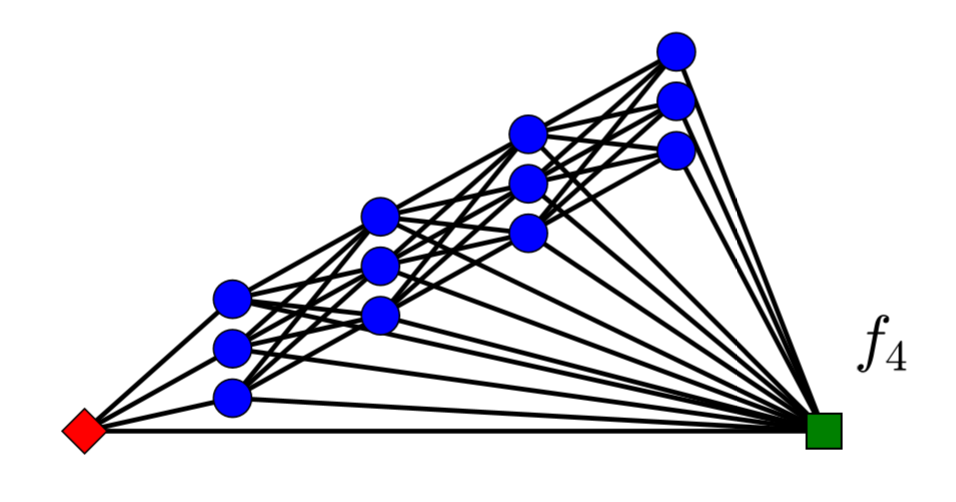
\includegraphics[width=1\textwidth]{f_4.png}
        \label{fig:figure2}
        \caption{ Realization of $f_{4}$. A feedforward neural network having $1$ input unit (diamond), $1$ output unit  (square), and $4\times 3=12$ units with ReLU activation (circles). }
    \end{figure}
\end{frame}

\subsubsection{Proposition 3.}
\begin{frame}{Proposition 3.}
    \begin{tcolorbox}
    \textbf{(Proposition 3.)}
        Given $M>0$ and $\varepsilon\in(0,1)$, there is a ReLU network $\eta$ with two input units that implements a function $\Tilde{x}:\mathbb{R}^{2}\rightarrow{\mathbb{R}}$ so that 
        \begin{itemize}
            \item for any inputs $x,y$, if $|x|\leq M$ and $|y|\leq M$, then  $|\Tilde{X}(x,y)-xy|\leq \varepsilon$;
            \item if $x=0$ or $y=0$, the $\Tilde{X}(x,y)=0$;
            \item the depth and the number of weights and computation units in $\eta$ is not greater than $c_{1}\ln(1/\varepsilon)+c_{2}$ with an absolute constant $c_{1}$ and a constant $c_{2}=c(M)$.
        \end{itemize}
    \end{tcolorbox}
    \textbf{Key idea}
    \begin{enumerate}
        \item Use a polarization identity : 
        \begin{equation*}
            xy = \frac{1}{2} \big( \underbrace{(x+y)^{2}}-\underbrace{x^{2}}-\underbrace{y^{2}} \big)
        \end{equation*}
        \item Approximate three underbraced terms with $f_m$ in Proposition 2. 
    \end{enumerate}
\end{frame}

\begin{frame}{Proof of Proposition 3.}
\begin{itemize}
    \item Let $\Tilde{f}_{\text{sq},\delta}$ be the approximate squaring function from Proposition 2 such that $\Tilde{f}_{\text{sq},\delta}(0)=0$ and $|\Tilde{f}_{\text{sq},\delta}(x)-x^{2}|<\delta$ for $x\in[0,1]$.
    \item WLOG set $M\geq 1$, for $|x|,|y|\leq M$, we have $|x+y|\leq 2M$. Using polarization identity, we can construct $\Tilde{X}(x,y)$ as follows:
    \begin{align*}
        \Tilde{X}(x,y) = 2M^{2}\bigg(\Tilde{f}_{\text{sq},\delta}\bigg(\frac{|x+y|^{2}}{2M}\bigg)
        - \Tilde{f}_{\text{sq},\delta}\bigg(\frac{|x|^{2}}{2M}\bigg) - \Tilde{f}_{\text{sq},\delta}\bigg(\frac{|y|^{2}}{2M}\bigg) \bigg)
    \end{align*}
    \item By setting $\delta = \frac{\varepsilon}{6M^{2}}$, we can get the error bound with $\varepsilon$ for any $\varepsilon\in [0,1]$, $|\Tilde{X}(x,y)-xy|\leq\varepsilon$.
    \item Construction of $\Tilde{X}$ only involves with three instances of $\Tilde{f}_{\text{sq},\delta}$ and finitely many linear and ReLU operations,
    \item Using Proposition 2, we can implement $\Tilde{X}$ by a ReLU network such that its depth and the number of computation units and weights $\mathcal{O}(\ln(1/\delta))$, which is $\mathcal{O}(\ln(1/\varepsilon)+\ln M)$.
\end{itemize}

\end{frame}

\section{Proof of Theorem 1.}
\subsection{First Step}
\begin{frame}{First Step}
    \begin{itemize}
    \item Neural Network $\Tilde{f}$ is not directly used to approximate $f\in\mathcal{W}^{n,\infty}([0,1]^{d})$, instead it is used to approximate the approximated $f$ through local Taylor expansion, where the paper denotes it as $f_{1}(X)$.
    \item For $X\in[0,1]^{d}$, the closeness between functions is measured in a $L^{\infty}$ sense. Approximation error can be decomposed with the help of triangular inequality as follows:
    \begin{eqnarray*}
        \scriptsize
        \left\| \Tilde{f} - f \right\|_{L^\infty[0,1]^{d}}
        \leq \underbrace{\left\| f_{1}(X) - f(X) \right\|_{L^\infty[0,1]^{d}}}_{\circled{1}} + 
        \underbrace{\left\| \Tilde{f}(x) - f_{1}(X) \right\|_{L^\infty[0,1]^{d}}}_{\circled{2}} .
    \end{eqnarray*}
    
    \item We want to control both terms $\circled{1}$ and $\circled{2}$ less than or equal to $\frac{\varepsilon}{2}$ respectively.
    In the first setp, we will focus on controlling $\circled{1}$.
    \end{itemize}
\end{frame}

\begin{frame}{Control on $\circled{1}$}
    \begin{itemize}
        \item  Recall that a function $f\in\mathcal{W}^{n,\infty}([0,1]^{d})$ is approximated via LTA with partition of unity formed by a grid of $(N+1)^{d}$ functions $\phi(m)$ for positive integer $N$: 
        \begin{equation*}
            \sum_{m} \underbrace{\prod_{j=1}^{d}\Psi(3N(x_{j}-m_{j}/N))}_{=\phi(m)} = 1, x \in [0,1]^{d},
        \end{equation*}
        where $m\in\{0,1,\dots,N\}^{d}$.
        \item  $\Psi(x)$ is the univariate trapezoid function :  $\Psi(x)=\sigma(x+2)-\sigma(x+1)-\sigma(x-1)+\sigma(x-2)$ supported on $[-2,2]$, equal to $1$ on $[-1,1]$, and linear on $[-2,-1] \cup [1,2]$.
    \end{itemize}
\end{frame}

\begin{frame}{Control on $\circled{1}$}
    \begin{itemize}
        \item The approximated function via Local Taylor Approximation, we can construct $f_{1}$ as follows:
        \begin{align*}
            f_{1}(x)
            &=\sum_{\textbf{m}\in\{0,1,\dots,N\}^{d}}\sum_{\alpha:|\alpha|\leq n-1}\frac{D^{\alpha}f\big(\frac{\textbf{m}}{N}\big)}{\alpha!}\phi(\textbf{m})\bigg(\textbf{x}-\frac{\textbf{m}}{N}\bigg)^{\alpha}
        \end{align*}
        \item We denote the degree-$(n-1)$ Taylor Polynomial for the function $f$ at $x=\frac{m}{N}$ as $P_m$, and rewrite $f_{1}(x)$ as follows :
        \begin{align*}
            f_{1}(x)&=\sum_{\textbf{m}\in\{0,1,\dots,N\}^{d}}\sum_{\alpha:|\alpha|\leq n-1}\frac{D^{\alpha}f\big(\frac{\textbf{m}}{N}\big)}{\alpha!}\bigg(\textbf{x}-\frac{\textbf{m}}{N}\bigg)^{\alpha}\phi(\textbf{m})\\
            &=\sum_{\textbf{m}\in\{0,1,\dots,N\}^{d}}P_{m}(x)\phi(\textbf{m}).
        \end{align*}
    \end{itemize}
\end{frame}

\begin{frame}{Control on $\circled{1}$}
    Observe $f(x)\in\mathcal{W}^{n,\infty}([0,1]^{d})$ can be written as follows by Multivariate Taylor's Theorem: for any $\xi \in [0,1]$ and any $a \in [0,1]^{d}$,
    \begin{equation*}
        \tiny
        f(x)=\sum_{\alpha:|\alpha|\leq n-1}D^{\alpha}f(a)\frac{(x-a)^{\alpha}}{\alpha!}+
        \sum_{\alpha:|\alpha|=n}D^{\alpha}f(a+\xi(x-a))\frac{(x-a)^{\alpha}}{\alpha!}.
     \end{equation*}
    Let $a=\frac{m}{N}$,
    \begin{align*}
        \left| f(x) - f_{1}(x) \right| = \left| \sum_{m}\phi_m(x) \big(f(x)-P_m(x)\big) \right|.
    \end{align*}
    In the above identity, we use the fact $\sum_{m}\phi_{m}(x)=1$ .
\end{frame}

\begin{frame}{Control on $\circled{1}$}
    \begin{align*}
        \left| \sum_{m}\phi_m(x) \big(f(x)-P_m(x)\big) \right|
        &\leq \sum_{m:|x_{k}-\frac{m_{k}}{N}|<\frac{1}{N}\forall k}
        \left| f(x)-P_m(x) \right|\\
        &\leq 2^{d}\max_{m:|x_{k}-\frac{m_{k}}{N}|<\frac{1}{N}\forall k}
        \left| f(x)-P_m(x) \right|\\
        &\leq \frac{2^{d} d^{n}}{n!}\bigg(\frac{1}{N}\bigg)^{n}
        \max_{\textbf{n}:|\textbf{n}|=n}\esssup_{x\in[0,1]^{d}}\left| D^{\textbf{n}}f(x) \right|\\
        &\leq \frac{2^{d} d^{n}}{n!}\bigg(\frac{1}{N}\bigg)^{n}.
    \end{align*}
    In the first inequality, we use the support condition of $\phi(m)$ and the fact $\|\phi_{m}\|_{\infty}=1$.
    In the second inequality, the fact that any $x\in[0,1]^{d}$ belongs to the support of at most $2^{d}$ functions $\phi_{m}$ is used. In the third, the standard bound for Taylor remainder and in the last inequality, the definition of $\mathcal{W}^{n,\infty}([0,1]^{d})$ are used.
\end{frame}

\begin{frame}{Control on $\circled{1}$}
    It follows that if we choose 
    \begin{equation*}
        N = \ceil{\big( \frac{n!}{2^{d}d^{n}} \frac{\varepsilon}{2} \big)^{-1/n}},
    \end{equation*}
    then the error follows 
    \begin{equation*}
        \| f - f_{1} \|_{\infty} 
        = \left| \sum_{m}\phi_m(x) \big(f(x)-P_m(x)\big) \right|
        \leq \frac{2^{d} d^{n}}{n!}\bigg(\frac{1}{N}\bigg)^{n}
        \leq \frac{\varepsilon}{2}.
    \end{equation*}
\end{frame}
\end{document}


